%\documentclass[fleqn]{article}
%\usepackage{graphicx} 
%\usepackage{here}    
%\usepackage{amsmath}
%\textwidth=15.0cm
%\textheight=22.0cm
%\topmargin=-1cm
%\oddsidemargin=-0.3cm
%\evensidemargin=-0.3cm
%
%
%%packages
%\usepackage{amsmath}
%\usepackage{cite}
%\usepackage[toc,page]{appendix}
%\usepackage{fancyvrb}
%\usepackage{tikz}
%\usepackage{multicol}
%\usepackage{framed}
%\usepackage{pgfplots}
%\usepackage{fixltx2e}
%\usepackage{subfigure}
%\usepackage{lscape}
%\usepackage{enumitem}
%\usepackage{multirow}
%\usepackage{color}
%\usepackage{xcolor}
%\usepackage{comment}
%\usepackage{changes}
%\renewcommand*\descriptionlabel[1]{\hspace\leftmargin$#1$}
%
%%tikz labraries
%\usetikzlibrary{matrix}
%\usetikzlibrary{decorations.pathreplacing}
%\usetikzlibrary{positioning}
%\usetikzlibrary{calc}
%\usetikzlibrary{shapes,arrows, chains}
%\usetikzlibrary{intersections}
%\usetikzlibrary{decorations.markings}
%\usetikzlibrary{calc,intersections}
%\usetikzlibrary{patterns}
%
%
%\makeatletter
%\def\mathcolor#1#{\@mathcolor{#1}}
%\def\@mathcolor#1#2#3{%
%  \protect\leavevmode
%  \begingroup
%    \color#1{#2}#3%
%  \endgroup
%}
%\makeatother
%
%%##### DEFINE YOUR NAME #########################
%\definechangesauthor[color=blue,name={Arpad Rozsas}]{AR}
%\definechangesauthor[color=red,name={Nadieh Meinen}]{NEM}
%%###########################################
%
%\begin{document}


\section{Case study}\label{case_study}

\subsection{Design situation}
A graphical summary of the (fictitious) design situation is presented in Figure \ref{tikz:design_situation}. The design situation exists of a  high-rise structure of height  $h=120$ m and a square plan with measurements of $w=b=30$ m. The structure is located at Schiphol Airport. All possible building orientations $\phi$ are investigated. The surrounding terrain roughness is equal to $z_0=0.8$ m. The faces of the building are named A to D. Interest goes to the fa\c{c}ade element located in the middle of face A at the height of $z=80$ m. The size of the fa\c{c}ade element is equal to  $A_{ref}=10$ m$^2$. The fa\c{c}ade element is designed for the EN1990 consequence class 2 (e.g. residential and office buildings) with the minimum design lifetime of $N=50$ years. The target value of the reliability index is equal to $\beta=3.8$. The detachment system of the fa\c{c}ade element is manufactured from steel and is loaded in axial compression. The incident wind-directions are discretized into sections of 30$^{\circ}$. 


\begin{figure}[H]
	\centering
	\subfigure[Location of the structure]{
		%\documentclass[fleqn]{report}
%\usepackage{graphicx} % om PostScript plaatje in te lassen
%\usepackage{here}     % voor geforceerde plaatsing figuren
%\usepackage{amsmath}
%\textwidth=17.0cm
%\textheight=22.0cm
%\topmargin=-1cm
%\oddsidemargin=-0.3cm
%\evensidemargin=-0.3cm
%
%%packages
%\usepackage{amsmath}
%\usepackage{cite}
%\usepackage[toc,page]{appendix}
%\usepackage{fancyvrb}
%\usepackage{tikz}
%\usepackage{multicol}
%\usepackage{framed}
%\usepackage{pgfplots}
%%\usepgfplotslibrary{fillbetween}
%\usepackage{fixltx2e}
%\usepackage{subfigure}
%\usepackage{lscape}
%\usepackage{enumitem}
%\usepackage{filecontents}
%\usetikzlibrary{decorations.pathmorphing}
%\usepackage{lmodern}
%\usepackage{pgfplotstable}
%
%\usetikzlibrary{arrows}
%%\usetikzlibrary{arrows.meta}
%
%
%
%\usetikzlibrary{decorations.pathreplacing,decorations.markings,snakes}
%
%%tikz labraries
%\usetikzlibrary{matrix}
%\usetikzlibrary{decorations.pathreplacing}
%\usetikzlibrary{positioning}
%\usetikzlibrary{calc}
%\usetikzlibrary{shapes,arrows, chains}
%\usetikzlibrary{patterns}
%
%\usetikzlibrary{intersections}
%\usetikzlibrary{decorations.markings}
%\usetikzlibrary{calc,intersections}
%%\usetikzlibrary{decorations.pathreplacing,bending}
%
%%extra instellingen
%\newlist{aims}{enumerate}{1}
%\setlist[aims,1]{
%  label={*},
%  leftmargin=*,
%  align=left,
%  labelsep=2mm,
%}
%
%\newlist{aims2}{enumerate}{1}
%\setlist[aims2,1]{
%  label={},
%  leftmargin=0pt,
%  align=left,
%  labelsep=4mm,
%}
%
%\newlist{aims3}{enumerate}{1}
%\setlist[aims3,1]{
%  label={-},
%  leftmargin=2cm,
%  align=left,
%  labelsep=0.4mm,
%}
%
%\usepackage{pgfplots}
%
%\begin{document}


\begin{tikzpicture}[scale=2]
\small 
\node [above right] (Nederland) at (0,0) {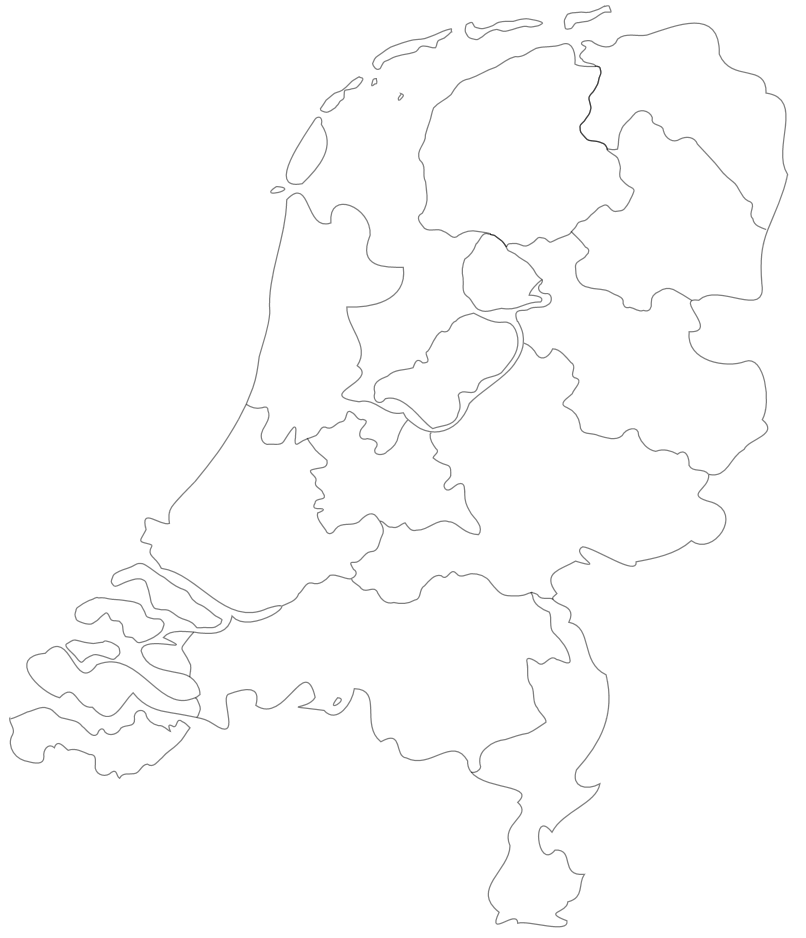
\includegraphics[height=4cm]{tikz/images/Nederland}};
\begin{scope}

\coordinate (schiphol) at (0.7,1.2);
\coordinate (vlissingen) at (0.15,0.57);
\coordinate (eindhoven) at (1,0.52);
%\coordinate (debilt) at (0.85, 1.0);

%\node [above](Eindhoven) at (eindhoven) {Eindhoven};
\node [above](Schiphol) at (schiphol) {Schiphol Airport};
%\node [above] (Vlissingen) at (vlissingen) {Vlissingen};
%\node [above](Debilt) at (debilt) {De Bilt};

\fill (schiphol) circle (0.2pt);
%\fill (eindhoven) circle (0.2pt);
%\fill (vlissingen) circle (0.2pt);
%\fill (debilt) circle (0.2pt);

\end{scope}



\end{tikzpicture}
%
%\end{document}
	}
	\subfigure[Location on the structure]{
		%
%\documentclass[fleqn]{report}
%\usepackage{graphicx} % om PostScript plaatje in te lassen
%\usepackage{here}     % voor geforceerde plaatsing figuren
%\usepackage{amsmath}
%\textwidth=17.0cm
%\textheight=22.0cm
%\topmargin=-1cm
%\oddsidemargin=-0.3cm
%\evensidemargin=-0.3cm
%
%%packages
%\usepackage{amsmath}
%\usepackage{cite}
%\usepackage[toc,page]{appendix}
%\usepackage{fancyvrb}
%\usepackage{tikz}
%\usepackage{multicol}
%\usepackage{framed}
%\usepackage{pgfplots}
%\usepackage{fixltx2e}
%\usepackage{subfigure}
%\usepackage{lscape}
%\usepackage{enumitem}
%\usepackage{filecontents}
%\usepackage{multicol}
%
%
%%tikz labraries
%\usetikzlibrary{matrix}
%\usetikzlibrary{decorations.pathreplacing}
%\usetikzlibrary{positioning}
%\usetikzlibrary{calc}
%\usetikzlibrary{shapes,arrows, chains}
%\usetikzlibrary{intersections}
%\usetikzlibrary{decorations.markings}
%\usetikzlibrary{calc,intersections}
%%\usetikzlibrary{decorations.pathreplacing,bending}
%
%% define mathcolor
%\makeatletter
%\def\mathcolor#1#{\@mathcolor{#1}}
%\def\@mathcolor#1#2#3{%
%  \protect\leavevmode
%  \begingroup
%    \color#1{#2}#3%
%  \endgroup
%}
%\makeatother
%
%%extra instellingen
%\newlist{aims}{enumerate}{1}
%\setlist[aims,1]{
%  label={*},
%  leftmargin=*,
%  align=left,
%  labelsep=2mm,
%}
%
%\newlist{aims2}{enumerate}{1}
%\setlist[aims2,1]{
%  label={},
%  leftmargin=0pt,
%  align=left,
%  labelsep=4mm,
%}
%
%\newlist{aims3}{enumerate}{1}
%\setlist[aims3,1]{
%  label={-},
%  leftmargin=2cm,
%  align=left,
%  labelsep=0.4mm,
%}
%
%\usepackage{pgfplots}
%
%\begin{document}

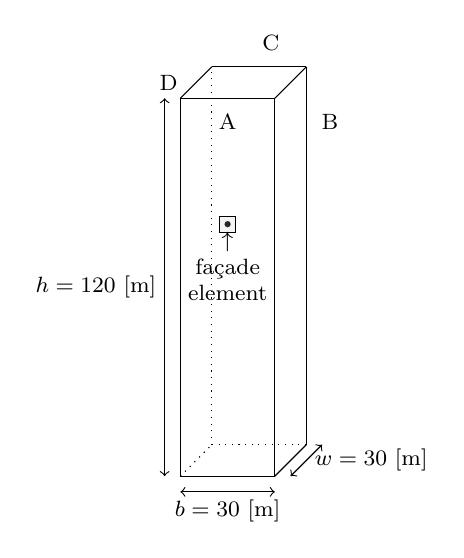
\begin{tikzpicture}[scale=10]
\footnotesize
\draw (-0.06,0) rectangle (0.06,0.480);
\draw (0.06,0) -- (0.10,0.04);
\draw (0.06,0.480) -- (0.10,0.52);
\draw (-0.06,0.480) -- (-0.02,0.52);
\draw (0.10,0.04) -- (0.10,0.52);
\draw (-0.02,0.52) -- (0.10,0.52);
\draw [dotted] (-0.06,0) -- (-0.02,0.04);
\draw [dotted] (-0.02,0.04) -- (0.1,0.04);
\draw [dotted] (-0.02,0.04) -- (-0.02,0.52);

% height
\draw [<->] (-0.08,0) -- (-0.08,0.480) node [midway, anchor=east] {$h = 120$ [m]};
% width
\draw [<->] (-0.06,-0.02) -- (0.06,-0.02) node [midway, anchor = north] {$b = 30$ [m]};
% depth
\draw [<->] (0.08,0) -- (0.12,0.04) node [midway, anchor = west] {$w = 30$ [m]};

%\draw [->] (-0.1,0) -- (-0.1,0.12);
%\node [left ] at  (-0.07,0.12) {$z$};
% x-distance
%\draw [<->] (-0.06,0.37) -- (0,0.37) node [midway, anchor = south] {x = 24 [m]};
% z-distance
%\draw [<->] (-0.03,0) -- (-0.03,0.32) node [midway, anchor = west] {$z = 80$ [m]};

\node at (0,0.45) {A};
\node at (0.13,0.45) {B};
\node at (0.055,0.55) {C};
\node at (-0.075,0.5) {D};
\draw (0,0.320) node[circle,fill,inner sep=0.8pt,align=center, label=below:]  (1) {};
\node [below, align=center] at (0,0.32) {$\uparrow$ \\ fa\c{c}ade \\ element};

\draw [fill=black!20, fill opacity=0.2] (-0.01,0.31) rectangle (0.01,0.33);


%\draw (-0.06,0.320) -- (0.06,0.32);
%\draw (0.06,0.320) --  (0.10,0.36); 


\end{tikzpicture}
%
%\end{document}
		\label{tikz:C_Okkebuilding_3D}
	}
	\subfigure[Orientation of the structure]{
		%
%\documentclass[fleqn]{report}
%\usepackage{graphicx} % om PostScript plaatje in te lassen
%\usepackage{here}     % voor geforceerde plaatsing figuren
%\usepackage{amsmath}
%\textwidth=17.0cm
%\textheight=22.0cm
%\topmargin=-1cm
%\oddsidemargin=-0.3cm
%\evensidemargin=-0.3cm
%
%%packages
%\usepackage{amsmath}
%\usepackage{cite}
%\usepackage[toc,page]{appendix}
%\usepackage{fancyvrb}
%\usepackage{tikz}
%\usepackage{multicol}
%\usepackage{framed}
%\usepackage{pgfplots}
%\usepackage{fixltx2e}
%\usepackage{subfigure}
%\usepackage{lscape}
%\usepackage{enumitem}
%\usepackage{filecontents}
%\usepackage{multicol}
%
%
%%tikz labraries
%\usetikzlibrary{matrix}
%\usetikzlibrary{decorations.pathreplacing}
%\usetikzlibrary{positioning}
%\usetikzlibrary{calc}
%\usetikzlibrary{shapes,arrows, chains}
%\usetikzlibrary{intersections}
%\usetikzlibrary{decorations.markings}
%\usetikzlibrary{calc,intersections}
%%\usetikzlibrary{decorations.pathreplacing,bending}
%
%% define mathcolor
%\makeatletter
%\def\mathcolor#1#{\@mathcolor{#1}}
%\def\@mathcolor#1#2#3{%
%  \protect\leavevmode
%  \begingroup
%    \color#1{#2}#3%
%  \endgroup
%}
%\makeatother
%
%%extra instellingen
%\newlist{aims}{enumerate}{1}
%\setlist[aims,1]{
%  label={*},
%  leftmargin=*,
%  align=left,
%  labelsep=2mm,
%}
%
%\newlist{aims2}{enumerate}{1}
%\setlist[aims2,1]{
%  label={},
%  leftmargin=0pt,
%  align=left,
%  labelsep=4mm,
%}
%
%\newlist{aims3}{enumerate}{1}
%\setlist[aims3,1]{
%  label={-},
%  leftmargin=2cm,
%  align=left,
%  labelsep=0.4mm,
%}
%
%\usepackage{pgfplots}
%
%\begin{document}

\begin{tikzpicture}[scale=1.3]
\footnotesize
\draw  (-1,-1) rectangle (1,1);
\draw  (0,-1) -- (0,1);
\draw  (-1,0) -- (1,0);
\draw [dotted,rotate around={15:(0,0)}] (-1,-1) rectangle (1,1);
\draw [dotted,rotate around={15:(0,0)}] (0,-1) -- (0,1);
\draw [dotted,rotate around={15:(0,0)}] (-1,0) -- (1,0);


\draw (-0.27,0.95) node[circle,fill,inner sep=0.8pt,align=center, label=below:]  (1) {};

\node [above, align=center] at (-0.27,0.95) {fa\c{c}ade \\ element \\ $\downarrow$ \\ };

\draw ([shift=(0:0cm)]0,0.6) arc (90:105:0.6cm);
\node [left] (nodela) at (-0.2,0.7) {$\phi$};

\draw (-1,-1) rectangle (1,1);
\node [left] at (-1,0.0) {B};
\node [right] at (1,0) {D};
\node [below] at (0,-1) {C};
\node [above] at (0,1) {A};


\begin{scope} [scale=0.7,shift={(3.5,2)}]
\coordinate (north) at (0,0.5);
\coordinate (east) at (0.5,0);
\coordinate (south) at (0,-0.5);
\coordinate (west) at (-0.5,0);

\draw [triangle 90-triangle 90] (north) -- (south);
\draw [triangle 90-triangle 90] (east) -- (west);
\node [above] (N) at (north) {N};
\node [right] (E) at (east) {E};
\node [below] (S) at (south) {S};
\node [left] (N) at (west) {W};
\end{scope}

\end{tikzpicture}

%\end{document}
	}
	\caption{Design situation}
	\label{tikz:design_situation}
\end{figure}






\subsection{Data under study}

\subsubsection{Wind speed data}
\begin{framed}
	To what extent will we mention that it matters how you discretize?
\end{framed}
For the probabilistic description of the $N$-yearly extreme wind speed, 'potential wind speed' parent data are used which are obtained from the KNMI-measurement station at Schiphol Airport. The potential wind speed data correspond to an hourly mean wind speed  at a reference height of $z_{ref}$ = 10 m and a standard terrain roughness of $z_{0,ref}$ = 0.03 m. The measurement period covers 64 years and the potential wind speeds are documented for every single hour. The accompanying incident wind-directions are documented for wind speed sections of $10^{\circ}$ which are combined to sections of $30^{\circ}$ (see Figure \ref{fig:incident_wind_directions}). 
A more detailed description of the wind speed data is provided in Meinen (2015).  


\subsubsection{Pressure coefficient data}\label{subsubsec:pressure_coefficient_data}
\begin{framed}
	To what extent will we mention that it matters how you discretize?
\end{framed}
For the description of the peak external pressure coefficients wind tunnel measurements are used which are obtained from the open-circuit atmospheric boundary layer wind tunnel of TNO with a full-scale terrain roughness $z_0=0.8$ m. The pressures are measured at taps placed at 172 locations on the building. In total two types of wind tunnel measurements are performed. The first type is called the 'long-run' experiment, where the incident flow is frontal only ($0^{\circ}\pm7.5^{\circ}$ for building orientation $\phi=0^{\circ}$), but of considerable long duration (approximately 175 hours in full scale). The second type is called the 'short-run' experiment, where the incident flow direction changed in sections of 15$^{\circ}$, but of shorter duration (approximately 30 minutes in full scale). The sections of $15^{\circ}$ are combined to sections of 30$^{\circ}$ (see Figure \ref{fig:incident_wind_directions2}). A more detailed description of the experimental materials, wind tunnel characteristics and executed measurements is provided in Meinen (2015).



\begin{figure}[H]
	\begin{minipage}[]{0.5\textwidth}
		%\documentclass[fleqn]{article}
%\usepackage{graphicx} % om PostScript plaatje in te lassen
%\usepackage{here}     % voor geforceerde plaatsing figuren
%\usepackage{amsmath}
%\textwidth=17.0cm
%\textheight=22.0cm
%\topmargin=-1cm
%\oddsidemargin=-0.3cm
%\evensidemargin=-0.3cm
%
%%packages
%\usepackage{amsmath}
%\usepackage{cite}
%\usepackage[toc,page]{appendix}
%\usepackage{fancyvrb}
%\usepackage{tikz}
%\usepackage{multicol}
%\usepackage{framed}
%\usepackage{pgfplots}
%\usepackage{fixltx2e}
%\usepackage{subfigure}
%\usepackage{lscape}
%\usepackage{enumitem}
%\usepackage{multirow}
%\usepackage{color}
%\renewcommand*\descriptionlabel[1]{\hspace\leftmargin$#1$}
%
%%tikz labraries
%\usetikzlibrary{matrix}
%\usetikzlibrary{decorations.pathreplacing}
%\usetikzlibrary{positioning}
%\usetikzlibrary{calc}
%\usetikzlibrary{shapes,arrows, chains}
%\usetikzlibrary{intersections}
%\usetikzlibrary{decorations.markings}
%\usetikzlibrary{calc,intersections}
%\usetikzlibrary{patterns}
%\usepackage{xcolor}
%
%%\usetikzlibrary{decorations.pathreplacing,bending}
%
%%extra instellingen
%\newlist{aims}{enumerate}{1}
%\setlist[aims,1]{
%  label={*},
%  leftmargin=*,
%  align=left,
%  labelsep=2mm,
%}
%
%\newlist{aims2}{enumerate}{1}
%\setlist[aims2,1]{
%  label={},
%  leftmargin=0pt,
%  align=left,
%  labelsep=4mm,
%}
%
%\newlist{aims3}{enumerate}{1}
%\setlist[aims3,1]{
%  label={-},
%  leftmargin=2cm,
%  align=left,
%  labelsep=0.4mm,
%}
%
%\makeatletter
%\def\mathcolor#1#{\@mathcolor{#1}}
%\def\@mathcolor#1#2#3{%
%  \protect\leavevmode
%  \begingroup
%    \color#1{#2}#3%
%  \endgroup
%}
%\makeatother
%
%
%% overige instellingen
%\makeatletter
%\newcommand\frontmatter{%
%    \cleardoublepage
%  \@mainmatterfalse
%  \pagenumbering{roman}}
%\newcommand\mainmatter{%
%    \cleardoublepage
%  \@mainmattertrue
%  \pagenumbering{arabic}}
%\newcommand\backmatter{%
%  \if@openright
%    \cleardoublepage
%  \else
%    \clearpage
%  \fi
% \@mainmatterfalse}
%\makeatother
%
%
%
%
%
%\begin{document}

\begin{tikzpicture}[scale=2.5]
\footnotesize

\filldraw[fill=black!20, rotate=-15] (0,1) arc (90:120:1cm);
\draw[black!20, fill=black!20, rotate=-15] (0,0) -- ($(0,0)!1cm!(0,1)$) to ($(0,0)!1cm!(-0.37,0.65)$)  -- cycle;

\begin{scope}[rotate=60]
\filldraw[fill=black!20, rotate=-15] (0,1) arc (90:120:1cm);
\draw[black!20, fill=black!20, rotate=-15] (0,0) -- ($(0,0)!1cm!(0,1)$) to ($(0,0)!1cm!(-0.37,0.65)$)  -- cycle;
\end{scope}

\begin{scope}[rotate=120]
\filldraw[fill=black!20, rotate=-15] (0,1) arc (90:120:1cm);
\draw[black!20, fill=black!20, rotate=-15] (0,0) -- ($(0,0)!1cm!(0,1)$) to ($(0,0)!1cm!(-0.37,0.65)$)  -- cycle;
\end{scope}

\begin{scope}[rotate=180]
\filldraw[fill=black!20, rotate=-15] (0,1) arc (90:120:1cm);
\draw[black!20, fill=black!20, rotate=-15] (0,0) -- ($(0,0)!1cm!(0,1)$) to ($(0,0)!1cm!(-0.37,0.65)$)  -- cycle;
\end{scope}

\begin{scope}[rotate=240]
\filldraw[fill=black!20, black=-15] (0,1) arc (90:120:1cm);
\draw[black!20, fill=black!20, rotate=-15] (0,0) -- ($(0,0)!1cm!(0,1)$) to ($(0,0)!1cm!(-0.37,0.65)$)  -- cycle;
\end{scope}

\begin{scope}[rotate=300]
\filldraw[fill=black!20, rotate=-15] (0,1) arc (90:120:1cm);
\draw[black!20, fill=black!20, rotate=-15] (0,0) -- ($(0,0)!1cm!(0,1)$) to ($(0,0)!1cm!(-0.37,0.65)$)  -- cycle;
\end{scope}


\draw (0,0) circle (1cm);


\begin{scope}[rotate=90]
\foreach \k in {0, 30, 60, 90, 120, 150, 180,  210,240, 270, 300, 330}
{
\node at (-\k:1.15) {\k $^{\circ}$};
}
\end{scope}




\foreach \i in {5, 15, 25, 35, 45, 55, 65, 75, 85, 95, 105, 115, 125, 135, 145, 155, 165, 175}
{
\draw [gray, rotate=\i] (0,-1) -- (0,1);
}

\foreach \i in {15, 45, 75, 105, 135, 165}
{
\draw [black, rotate=\i] (0,-1) -- (0,1);
}



\begin{scope}[shift={(1.5,0.7)}, scale=0.15]
\coordinate (north) at (0,1);
\coordinate (south) at (0,-1);
\coordinate (east) at (1,0);
\coordinate (west) at (-1,0);
\draw [triangle 90-triangle 90] (north) -- (south);
\draw [triangle 90-triangle 90] (east) -- (west);
\node [above] (N) at (north) {N};
\node [right] (E) at (east) {E};
\node [below] (S) at (south) {S};
\node [left] (N) at (west) {W};
\end{scope}

\end{tikzpicture}

%\end{document}
		\caption{Discretized incident wind-directions for sections of 30$^{\circ}$ - wind speeds}
		\label{fig:incident_wind_directions}
	\end{minipage}
	\hspace{0.4cm}
	\begin{minipage}[]{0.5\textwidth}
		%\documentclass[fleqn]{report}
%\usepackage{graphicx} % om PostScript plaatje in te lassen
%\usepackage{here}     % voor geforceerde plaatsing figuren
%\usepackage{amsmath}
%\textwidth=17.0cm
%\textheight=22.0cm
%\topmargin=-1cm
%\oddsidemargin=-0.3cm
%\evensidemargin=-0.3cm
%
%%packages
%\usepackage{amsmath}
%\usepackage{cite}
%\usepackage[toc,page]{appendix}
%\usepackage{fancyvrb}
%\usepackage{tikz}
%\usepackage{multicol}
%\usepackage{framed}
%\usepackage{pgfplots}
%%\usepgfplotslibrary{fillbetween}
%\usepackage{fixltx2e}
%\usepackage{subfigure}
%\usepackage{lscape}
%\usepackage{enumitem}
%\usepackage{filecontents}
%\usetikzlibrary{decorations.pathmorphing}
%\usepackage{lmodern}
%\usepackage{pgfplotstable}
%
%\usetikzlibrary{arrows}
%%\usetikzlibrary{arrows.meta}
%
%
%
%\usetikzlibrary{decorations.pathreplacing,decorations.markings,snakes}
%
%%tikz labraries
%\usetikzlibrary{matrix}
%\usetikzlibrary{decorations.pathreplacing}
%\usetikzlibrary{positioning}
%\usetikzlibrary{calc}
%\usetikzlibrary{shapes,arrows, chains}
%\usetikzlibrary{patterns}
%
%\usetikzlibrary{intersections}
%\usetikzlibrary{decorations.markings}
%\usetikzlibrary{calc,intersections}
%%\usetikzlibrary{decorations.pathreplacing,bending}
%
%%extra instellingen
%\newlist{aims}{enumerate}{1}
%\setlist[aims,1]{
%  label={*},
%  leftmargin=*,
%  align=left,
%  labelsep=2mm,
%}
%
%\newlist{aims2}{enumerate}{1}
%\setlist[aims2,1]{
%  label={},
%  leftmargin=0pt,
%  align=left,
%  labelsep=4mm,
%}
%
%\newlist{aims3}{enumerate}{1}
%\setlist[aims3,1]{
%  label={-},
%  leftmargin=2cm,
%  align=left,
%  labelsep=0.4mm,
%}
%
%\usepackage{pgfplots}
%
%\begin{document}
%\begin{figure}
%\centering
%
%





\begin{tikzpicture}[scale=2.5]

\footnotesize

\begin{scope}[rotate=-22.5]

\filldraw[fill=black!10] (0,1) arc (90:120:1cm);
\draw[black!10, fill=black!10] (0,0) -- ($(0,0)!1cm!(0,1)$) to ($(0,0)!1cm!(-0.37,0.65)$)  -- cycle;

\begin{scope}[rotate=60]
\filldraw[fill=black!10] (0,1) arc (90:120:1cm);
\draw[black!10, fill=black!10] (0,0) -- ($(0,0)!1cm!(0,1)$) to ($(0,0)!1cm!(-0.37,0.65)$)  -- cycle;
\end{scope}

\begin{scope}[rotate=120]
\filldraw[fill=black!10] (0,1) arc (90:120:1cm);
\draw[black!10, fill=black!10] (0,0) -- ($(0,0)!1cm!(0,1)$) to ($(0,0)!1cm!(-0.37,0.65)$)  -- cycle;
\end{scope}

\begin{scope}[rotate=180]
\filldraw[fill=black!10] (0,1) arc (90:120:1cm);
\draw[black!10, fill=black!10] (0,0) -- ($(0,0)!1cm!(0,1)$) to ($(0,0)!1cm!(-0.37,0.65)$)  -- cycle;
\end{scope}

\begin{scope}[rotate=240]
\filldraw[fill=purple!10] (0,1) arc (90:120:1cm);
\draw[black!10, fill=black!10] (0,0) -- ($(0,0)!1cm!(0,1)$) to ($(0,0)!1cm!(-0.37,0.65)$)  -- cycle;
\end{scope}

\begin{scope}[rotate=300]
\filldraw[fill=black!10] (0,1) arc (90:120:1cm);
\draw[black!10, fill=black!10] (0,0) -- ($(0,0)!1cm!(0,1)$) to ($(0,0)!1cm!(-0.37,0.65)$)  -- cycle;
\end{scope}
\end{scope}

\begin{scope}[rotate=7.5]
\foreach \i in {0, 15, 30, 45, 60, 75, 90, 105, 120, 135, 150, 165, 180, 195, 210, 225, 240, 255, 270, 285, 300, 315, 330, 345}
{
\draw [gray, rotate=\i] (0,-1) -- (0,1);
}
\foreach \i in {0, 30, 60, 90, 120, 150, 180, 210, 240, 270, 300, 330}
{
\draw [black, rotate=\i] (0,-1) -- (0,1);
}
\end{scope}

\draw (0,0) circle (1cm);


\begin{scope}[rotate=90]
\foreach \k in {0, 15, 30, 45, 60, 75, 90, 105, 120, 135, 150, 165, 180, 195, 210, 225, 240, 255, 270, 285, 300, 315, 330, 345}
{
\node at (-\k:1.15) {\k $^{\circ}$};
}
\end{scope}


\begin{scope}[scale=0.3]
\begin{scope}[shift={(0,-1)}]
\footnotesize
\draw [fill=white] (-1, -1) rectangle (1,1);
\draw [fill=black] (0, 1) circle (0.1);
\node [below, align=center] at (0,1) {$\uparrow$ \\ fa\c{c}ade \\ element};
\end{scope}
\end{scope}


\end{tikzpicture}

%\end{figure}
%
%\end{document}
		\caption{Discretized incident wind-directions for sections of 30$^{\circ}$ - pressure coefficients}
		\label{fig:incident_wind_directions2}
	\end{minipage}
\end{figure}




\subsection{Derivation probabilistic models}
First step is to obtain the probabilistic models for each of the parameters mentioned in PARAGRAPH.


\subsubsection{Structural resistance}
Step by step explanation on how the distribution function..

First step is to determine the design value of the load effects as 

Mayybe first we need to explain how the design value oft he structural resistance is obtained. That was missing in my previous paper. \\
\\
First step is to determine the design value of the structural resistance... Here we use




This limits to the data
\subsubsection{Probabilistic description of the extreme wind speeds}
\begin{framed}
Codification of wind load for structural design requires the estimation of the quantiles or return period values of the annual maximum wind speed. The wind speed of interest can be the hourly-mean wind speed [1] or the gust wind speed (ASCE-07). Given wind records, the tasks of extreme value analysis of wind speed for a single meteorological station are: the extraction of necessary number of samples of maximum wind speed from the wind records with/without an imposed threshold; the choice of probabilistic model (e.g., the selection of probability distribution type); and the extreme value analysis using the selected model and extracted data. The peak or maximum wind speed data can be extracted based on several criteria: maximum per specified time interval (e.g., per year), over a specified threshold, or the r-th largest values. The major advantage of using annual extreme values is the simplicity in data processing, although its use potentially reduces the amount of available wind data that can be considered for extreme analysis. The use of the r-th largest order statistics [2], and the data over a peak threshold can ameliorate the data scarcity, but the results could be sensitive to the size of r and the threshold selected. Moreover, if multiyear and multi-station data are considered, significant efforts are needed to process and inspect the data and to ensure that they are from independent events.

Extreme value analysis of the annual maximum wind speed at a site by using different probabilistic models was presented and debated (e.g., Refs. [3–7]). It seems that the Gumbel distribution is the most widely used probabilistic model for extreme value wind speed analysis [8–11]. This distribution has no upper bound, although use of a distribution without finite upper end point for extreme wind speed has been criticized on thermodynamic ground, but a justifiable finite upper end point is unclear. The distribution fitting methods used include the method of moments, the method of the maximum likelihood, the generalized least-squares, and the method of L-moments (MLM) [12]. The use of the generalised Pareto distribution and the generalized extreme value (GEV) distribution to maximum wind speeds has also been considered [4,13]. The application of generalised Pareto distribution is debated [4,5,7]. For the wind speed data from 235 meteorological stations in Canada, the at-site extreme value analysis results and the calculated values of the Akaike information criterion (AIC) [14] indicate that the Gumbel model for majority of stations outperforms the GEV distribution [15].
\end{framed}




According to paragraph \ref{subsubsec:windpseeds}, for each incident wind-direction the yearly extreme hourly mean wind speeds are obtained, resulting in 64 extremes for each incident wind-direction. Table \ref{table:tab:V_sample_statistics_max}                                                            column 2-5  provides the numerical summaries of the extremes, where $\hat{\mu}_v$ indicates the sample mean, $\hat{\text{V}}_v$ the sample variance and $\hat{\alpha}_v$  the sample skewness. The characteristics of the yearly extreme hourly mean wind speeds differ greatly for the distinct incident wind-directions. E.g. the sample mean $\hat{\mu}_v$ variates between 10.1 m/s for $\theta_i=120^{\circ}$ to 19.7 m/s for $\theta_i=240^{\circ}$. Thereby the highest mean wind speeds are found between $210^{\circ}\leq \theta_i\leq 270^{\circ}$, representing the winds coming from the South-West direction. The sample coefficient of variation $\hat{\text{V}}_v$ variates between 0.12   for $\theta_i=210^{\circ}$ and 0.18 for $\theta_i=0^{\circ}$. The sample skewness $\hat{\alpha}_v$ variates between 0.44  for $\theta_i=270^{\circ}$ and 1.56 for $\theta_i=120^{\circ}$. It is also observed that the parent wind coming from incident wind-direction $\theta_i$ is not uniformly distributed throughout the wind-rose; wind speeds coming from the South-West direction clearly have a higher probability of occurrence than the wind speeds coming from other directions. 


\begin{table}[H]                                                                                     
	\footnotesize
	\centering                                                                                            
	\caption{Numerical summaries and Gumbel model parameters of the yearly extreme hourly mean wind speeds as a function of the incident wind-direction $\theta_i$}
	\label{table:tab:V_sample_statistics_max}                                                             
	\begin{tabular}{|c|c|c|c|c|c|c|}                                                                    
		\hline
		&  \multicolumn{4}{|c|}{numerical summaries}             & \multicolumn{2}{|c|}{Gumbel model parameters} \\ \hline                                                                                              
		$\theta_i\pm15^{\circ}$ &	$\hat{\mu_v}$	&	$\hat{\text{V}}_v$	&	$\hat{\alpha}_v$	&	$p(\theta_i)$	&	$\alpha$	&	$u$	\\	\hline
		0$^{\circ}$	&	13.2	&	\textbf{0.18}	&	0.76	&	0.06	&	0.51	&	12.07	\\	\hline
		30$^{\circ}$	&	12.4	&	0.13	&	0.59	&	0.06	&	0.77	&	11.69	\\	\hline
		60$^{\circ}$	&	12.6	&	0.14	&	0.64	&	0.08	&	0.68	&	11.79	\\	\hline
		90$^{\circ}$	&	11.1	&	0.18	&	1.16	&	0.07	&	0.67	&	10.26	\\	\hline
		120$^{\circ}$	&	\textbf{10.1}	&	0.16	&	\textbf{1.56}	&	0.05	&	0.86	&	9.41	\\	\hline
		150$^{\circ}$	&	11.8	&	0.14	&	0.70	&	0.07	&	0.73	&	11.04	\\	\hline
		180$^{\circ}$	&	14.3	&	0.14	&	0.91	&	0.10	&	0.62	&	13.35	\\	\hline
		210$^{\circ}$	&	17.6	&	\textbf{0.12}	&	0.95	&	0.14	&	0.56	&	16.63	\\	\hline
		240$^{\circ}$	&	\textbf{19.7}	&	0.14	&	0.52	&	0.12	&	0.43	&	18.42	\\	\hline
		270$^{\circ}$	&	18.3	&	0.17	&	\textbf{0.44}	&	0.10	&	0.38	&	16.81	\\	\hline
		300$^{\circ}$	&	17.2	&	0.17	&	0.77	&	0.07	&	0.41	&	15.83	\\	\hline
		330$^{\circ}$	&	15.4	&	0.17	&	1.40	&	0.07	&	0.53	&	14.23	\\	\hline
	\end{tabular}
\end{table}

% illustration
\begin{figure}[H] 
	\centering    
	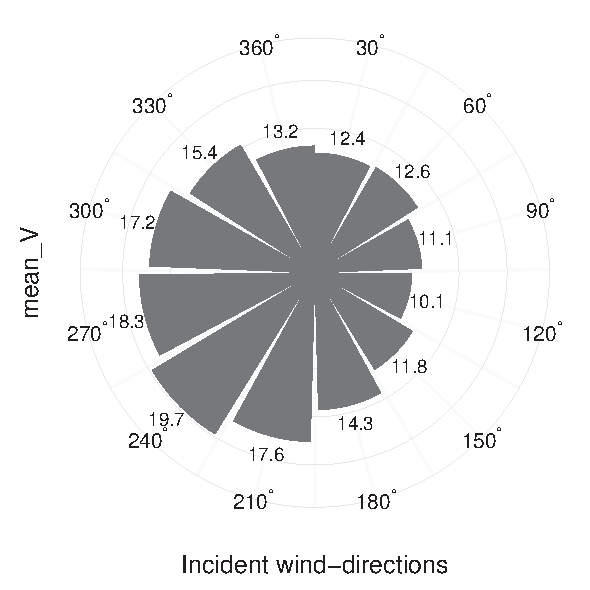
\includegraphics[width=0.4\textwidth]{images/Schiphol_mean_V_test.pdf}
	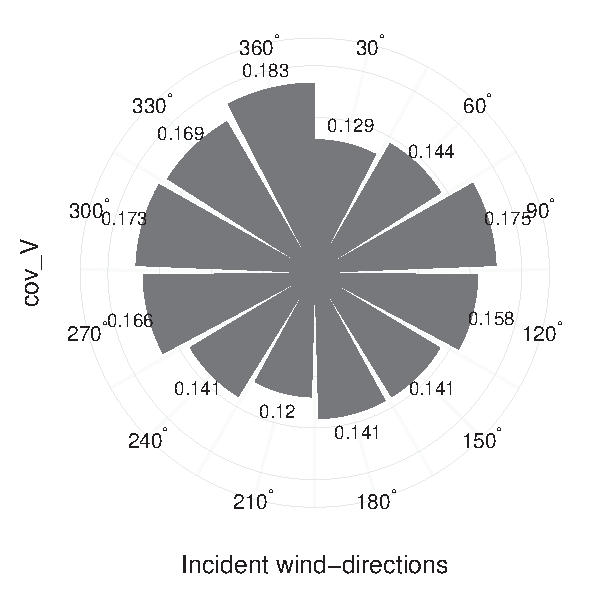
\includegraphics[width=0.4\textwidth]{images/Schiphol_cov_V_test.pdf}
	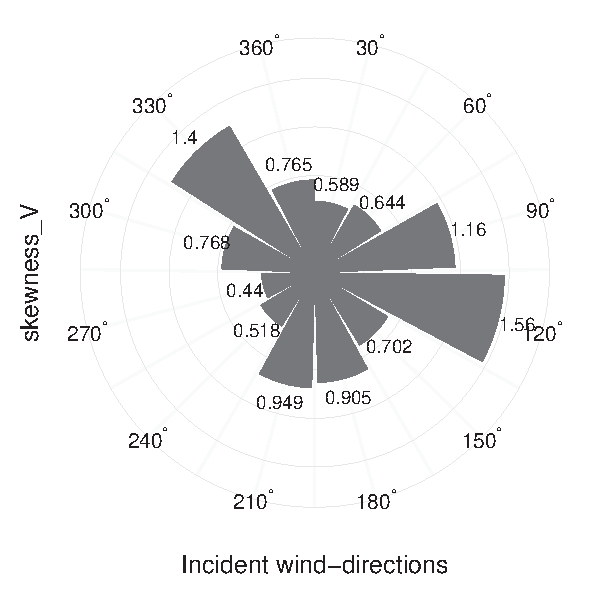
\includegraphics[width=0.4\textwidth]{images/Schiphol_skewness_V_test.pdf}
	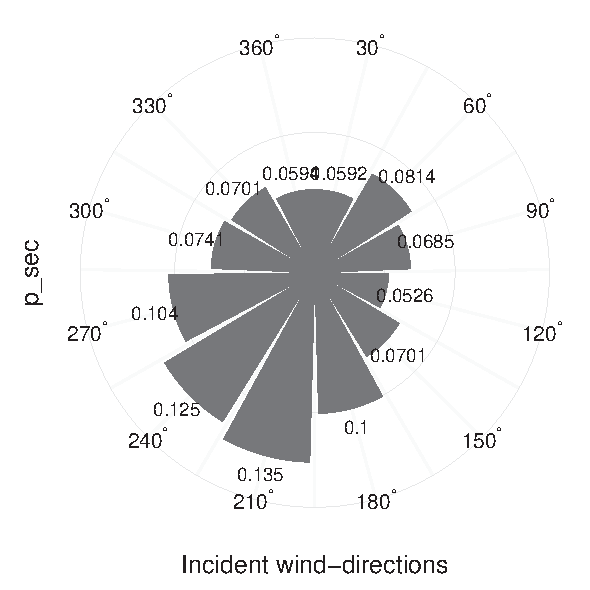
\includegraphics[width=0.4\textwidth]{images/Schiphol_p_sec_test.pdf}
	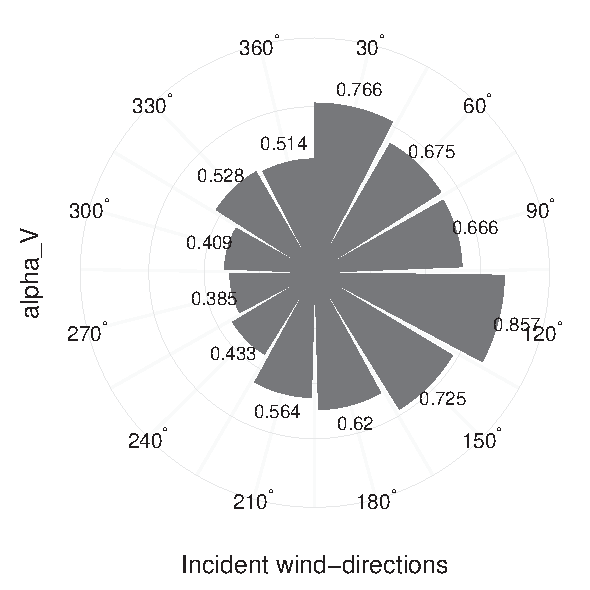
\includegraphics[width=0.4\textwidth]{images/Schiphol_alpha_V_test.pdf}
	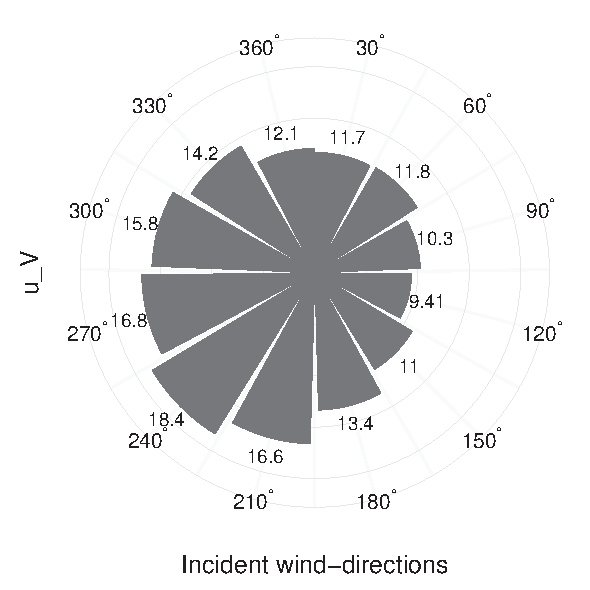
\includegraphics[width=0.4\textwidth]{images/Schiphol_u_V_test.pdf}
	\caption{Numerical summaries and Gumbel model parameters of the yearly extreme hourly mean wind speeds as a function of the incident wind-direction $\theta_i$}
	\label{fig:compass_summary_wind}
\end{figure}

\noindent
For each incident wind-direction the Gumbel distribution is fitted on the yearly extreme hourly mean wind speeds. The parameters of the Gumbel distribution are provided in table \ref{table:tab:V_sample_statistics_max} column 6-7.                                                       
Figure \ref{figure_V_240} and \ref{figure_V_270} show the model distribution functions together with the sample data for the governing incident wind-directions, plotted in the Gumbeldomain. 
It is observed that, towards the higher probability fractiles, the discrepancy between the sample data and the distribution function increases. 


\begin{figure}[H]
	\begin{minipage}[]{0.5\textwidth}
		\centering
		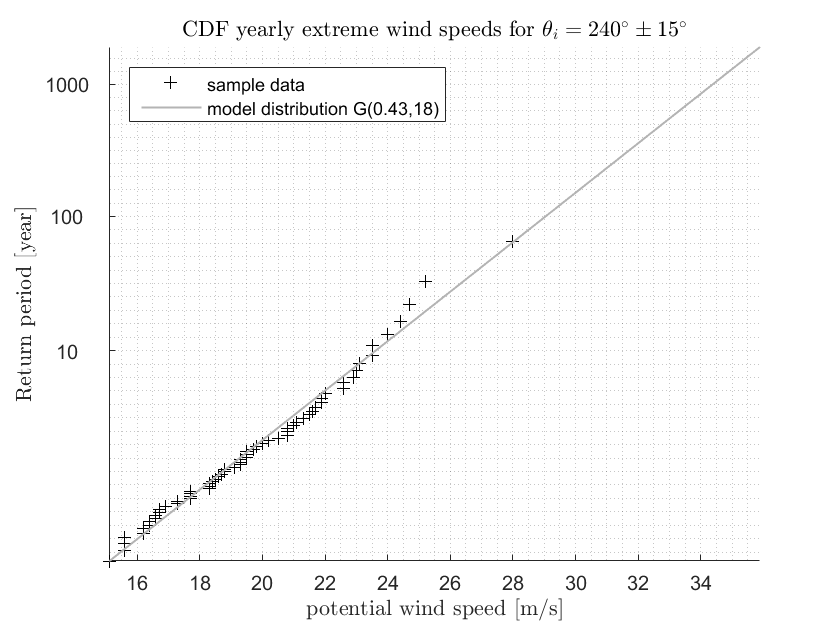
\includegraphics[scale=0.4]{images/CDF_yearly_extreme_windspeeds_G}
		\caption{Cumulative distribution  function (CDF) of the yearly extreme hourly mean wind speeds for $\theta_i=240^{\circ}\pm 15^{\circ}$}
		\label{figure_V_240}
	\end{minipage}
	\hspace{0.4cm}
	\begin{minipage}[]{0.5\textwidth}
		\centering
		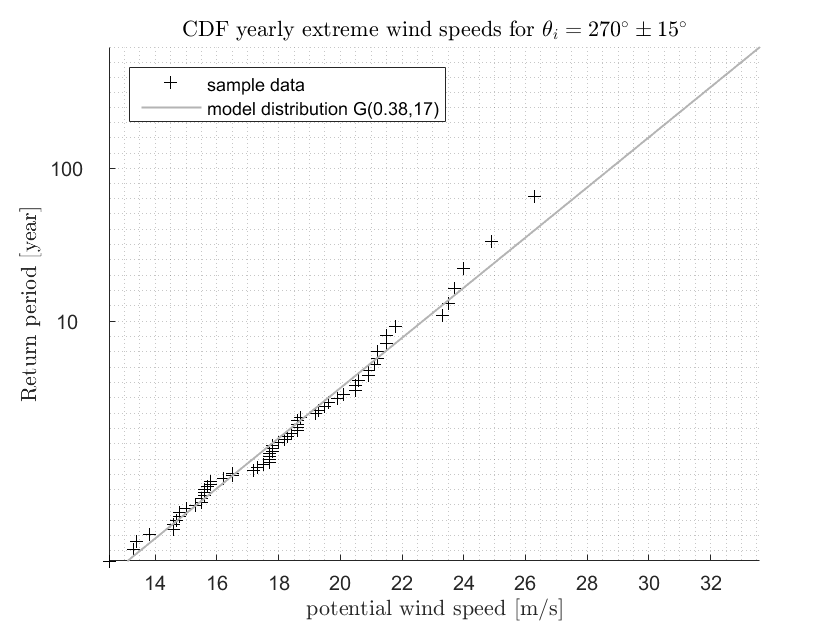
\includegraphics[scale=0.4]{images/CDF_yearly_extreme_windspeeds_G270}
		\caption{Cumulative distribution function (CDF) of the yearly extreme hourly mean wind speeds for $\theta_i=270^{\circ}\pm 15^{\circ}$}
		\label{figure_V_270}
	\end{minipage}
\end{figure}

\subsubsection{Probabilistic description of the hourly extreme pressure coefficients}
For the determination of the minimum required block-duration $t$ use is made of the 175 hour 'long run' wind tunnel data. In Meinen (2015) it was found that the value $t$ where the envelope autocorrelation function is equal to $R_{xx}(t)\leq0.2$ is approximately $t=10$ s. The block-duration chosen for further analysis is therefore $t=10$ s. \\
\\
Based on the 30 minutes 'short-run' wind-tunnel data for each incident wind-direction the the 10s-extreme peak external pressure coefficients are obtained, both for the maxima ($\hat{c}_{pe}$) and for the minima ($\check{c}_{pe}$), resulting in $2\cdot180$ extremes for each incident wind-direction. By analyzing the characteristics of the sample data it was observed that for the incident wind-directions
$\theta_i=7.5^{\circ}$, $\theta_i=37.5^{\circ}$ and $\theta_i=307.5^{\circ}$ and $\theta_i=337.5^{\circ}$ the maxima were governing, where for all other incident wind-directions the minima were governing. Table \ref{table:descriptive_statistics_C}                                                              provides the numerical summaries of the 10s-extreme peak external pressure coefficients for each incident wind-direction $\theta_i$ accordingly. In the table $\hat{\mu}_c$ indicates the sample mean, $\hat{\text{V}}_c$ indicates the unbiased sample coefficient of variation and $\hat{\alpha}_c$ the sample skewness. On average, the highest maxima are found for incident wind-direction $\theta_i=7.5^{\circ}$, of which the mean is equal to $\mu_{c}=1.1$. On average, the highest minima are found for incident wind-direction $\theta_i=277.5^{\circ}$, of which the mean is equal to $\mu_{c}=-1.3$. The coefficient of variation $\hat{\text{V}}_{c}$ variates between 0.12 for incident wind-direction $\theta_i=217.5^{\circ}$ and 0.36 for incident wind-direction $\theta=67.5^{\circ}$. The sample skewness $\hat{\alpha}_c$ variates between -1.65  for incident wind-direction $\theta=247.5^{\circ}$ and 0.16  for incident wind-direction $\theta=37.5^{\circ}$.  \\
\\
It is remarked that the highest extremes are found for incident wind-direction $\theta_i=67.5^{\circ}$ and not for incident wind-direction $\theta_i=277.5^{\circ}$. This is attributed to the fact that the coefficient of variation of incident wind-direction $\theta_i=67.5^{\circ}$ is larger than the coefficient of variation for incident wind-direction $\theta_i=277.5^{\circ}$. 



\begin{table}[H]                                                                                     
	\footnotesize
	\centering                                                                                            
	\caption{Numerical summaries and Gumbel model parameters of the 10s extreme peak external pressure coefficients as a function of the incident wind-direction $\theta_i$}
	\label{table:descriptive_statistics_C}                                                             
	\begin{tabular}{|c|c|c|c|c|c|c|}                                                                    
		\hline
		&               &\multicolumn{3}{|c|}{numerical summaries}  &\multicolumn{2}{|c|}{model parameters}             \\ \hline
		$\theta_i\pm15^{\circ}$	&	max/min	&	$\hat{\mu_c}$	&	$\hat{\text{V}}_c$ &	$\hat{\alpha}_c$	&	$\alpha$	&	$u$	\\	\hline
		7.5$^{\circ}$	&	max	&	\textbf{1.1}	&	0.13	&	-0.40	&	6.49	&	1.06	\\	\hline
		37.5$^{\circ}$	&	max	&	0.9	&	0.20	&	\textbf{0.16}	&	6.22	&	0.78	\\	\hline
		67.5$^{\circ}$	&	min	&	-1.0	&	\textbf{0.36}	&	0.06	&	2.83	&	-0.82	\\	\hline
		97.5$^{\circ}$	&	min	&	-1.2	&	0.24	&	-0.68	&	4.28	&	-1.05	\\	\hline
		127.5$^{\circ}$	&	min	&	-0.6	&	0.12	&	-0.43	&	16.92	&	-0.54	\\	\hline
		157.5$^{\circ}$	&	min	&	-0.6	&	0.12	&	-0.49	&	17.21	&	-0.52	\\	\hline
		187.5$^{\circ}$	&	min	&	-0.5	&	0.19	&	-0.89	&	11.97	&	-0.48	\\	\hline
		217.5$^{\circ}$	&	min	&	-0.5	&	\textbf{0.12}	&	-0.34	&	16.01	&	-0.50	\\	\hline
		247.5$^{\circ}$	&	min	&	-0.7	&	0.18	&	\textbf{-1.65}	&	11.29	&	-0.61	\\	\hline
		277.5$^{\circ}$	&	min	&	\textbf{-1.3}	&	0.21	&	-0.36	&	4.13	&	-1.15	\\	\hline
		307.5$^{\circ}$	&	max	&	0.6	&	0.24	&	0.14	&	7.8	&	0.53	\\	\hline
		337.5$^{\circ}$	&	max	&	1.1	&	0.15	&	0.11	&	6.73	&	0.98	\\	\hline
	\end{tabular}
\end{table}

\noindent
For each incident wind-direction the Gumbel distribution is fitted on the 10s-extreme peak external pressure coefficients. 
The parameters of the Gumbel distribution are provided in Table 
\ref{table:descriptive_statistics_C}                                                              column 6-7. Figure \ref{fig:C_maxima} and \ref{fig:C_minima} show respectively the model distributions of the 10s-maximum and 10s-minimum peak external pressure coefficients for the governing incident wind-directions, plotted in the Gumbeldomain. The sample data show a curved behaviour in the Gumbeldomain. As a consequence, in the higher probability fractiles, the Gumbel distributions (which show a straight line in the Gumbeldomain by definition) deviate significantly from the sample data. A similar behaviour is found for most other incident wind-directions. 

\begin{figure}[H]
	\begin{minipage}[]{0.5\textwidth}
		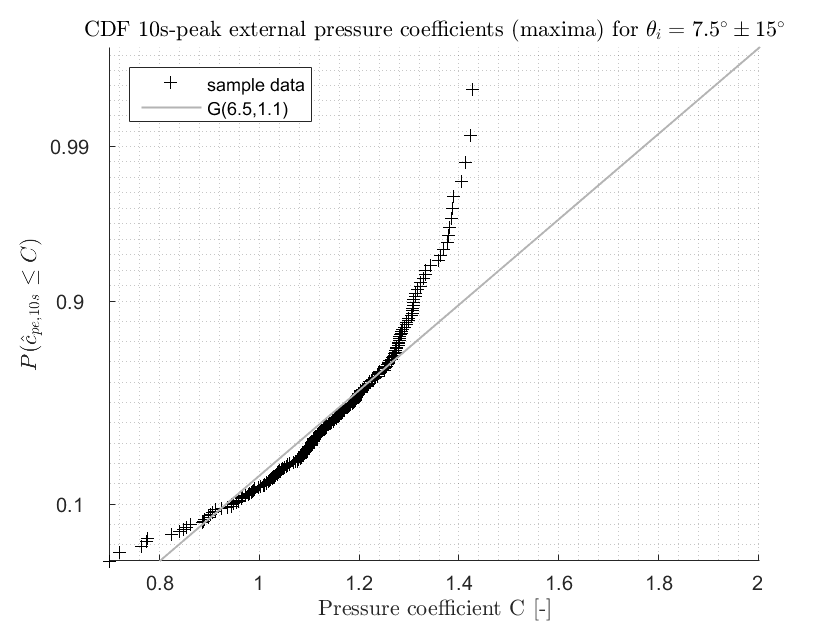
\includegraphics[scale=0.4]{images/CDF_10s_peak_external_pressure_coefficients_maxima_G}
		\caption{Cumulative distribution function (CDF) of the 10s-maximum peak external pressure coefficients for incident wind-direction $\theta_i=7.5^{\circ}\pm15^{\circ}$} \label{fig:C_maxima}
	\end{minipage}
	\hspace{0.4cm}
	\begin{minipage}[]{0.5\textwidth}
		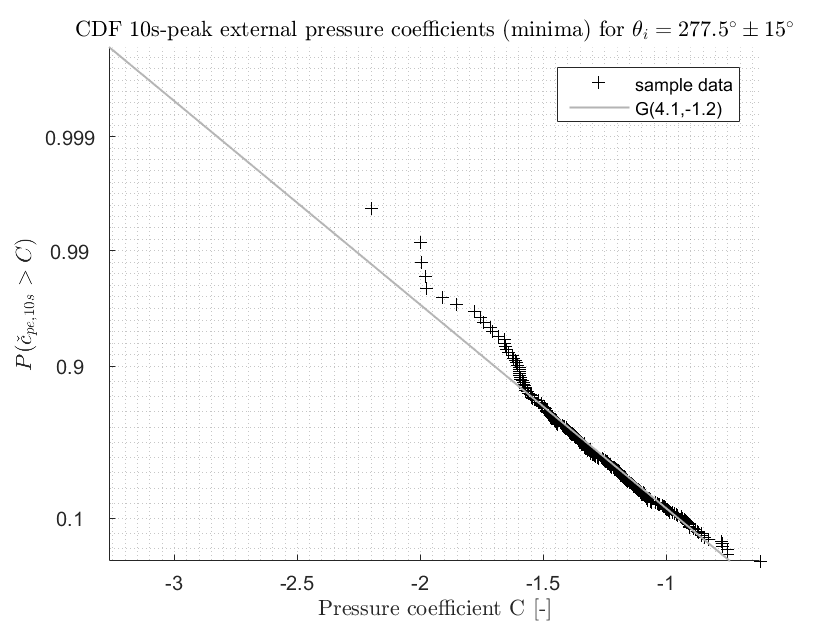
\includegraphics[scale=0.4]{images/CDF_10s_peak_external_pressure_coefficients_minima_G}
		\caption{Cumulative distribution function (CDF) of the 10s-minimum peak external pressure coefficients for incident wind-direction $\theta_i=277.5^{\circ}\pm15^{\circ}$} \label{fig:C_minima}
	\end{minipage}
\end{figure}



\subsubsection{Results reliability calculations}
For each building orientation $\phi$ the total failure probability of the fa\c{c}ade element is determined according to equations \ref{limit_state_function} to \ref{beta_total}. Figure \ref{fig:total_reliability_all_directiosn} shows  the resulting reliability indices $\beta_{total}$. The figure shows that the structural reliability is strongly dependent on the building orientation. Reliability indices are found between $\beta_{total}= 3.1$ for the governing building orientation $\phi=187.5^{\circ}$ and $\beta_{total}=4.6$ for the most advantageous building orientation $\phi=277.5^{\circ}$. It is remarked that the governing building orientation is that orientation where the  governing wind speeds (coming from incident wind-direction $\theta_i=240^{\circ}$) are combined with the governing peak external pressure coefficients (coming from incident wind-direction $\theta_i= 67.5^{\circ}$).\\
\\
Figure \ref{fig:direction_dependent_beta_values} shows the direction-dependent unconditional $\beta$-values for the governing building orientation $\phi=187.5^{\circ}$. Additionally the figure shows $\beta_{total}$ plotted as a horizontal black line. The direction-dependent unconditional $\beta$-values differ greatly for the incident wind-directions. Unconditional $\beta$-values are found between $\beta(\theta_i)=3.1$ for $\theta_i=240^{\circ}$ to $\beta(\theta_i)> 8$ for $\theta_i=30^{\circ}$. In terms of the failure probability, this differs several orders of magnitude. Consequentially, the total structural reliability is almost fully determined by incident wind-direction $\theta=240^{\circ}$ only;  the influence of all other incident wind-directions is negligibly small. A similar one-direction dominance is found for all other building orientations. In most cases the dominant incident wind-direction lies within $210^{\circ} \leq\theta_i \leq 270^{\circ}$, representing the wind speeds coming from the South-West direction.\\
\\
Table \ref{alpha-values} shows the averaged sensitivity factors ($\alpha$-values) for all incident wind-directions and all orientations of the building. The $\alpha$-values are highest for the hourly extreme wind speeds, with an average of $\alpha_{v_{hr,N}} = -0.83$. The $\alpha$-values are lowest for the structural resistance and the model uncertainty factor, with $\alpha_R=0.22$ and $\alpha_{\chi_{model}}=-0.20$ respectively. It is remarked that the observed $\alpha_R$-value of the structural resistance lies far from the chosen $\alpha_R=0.8$ in subsection \ref{sec:as}. 





\begin{figure}[H]
	\begin{minipage}[]{0.5\textwidth}
		\centering
		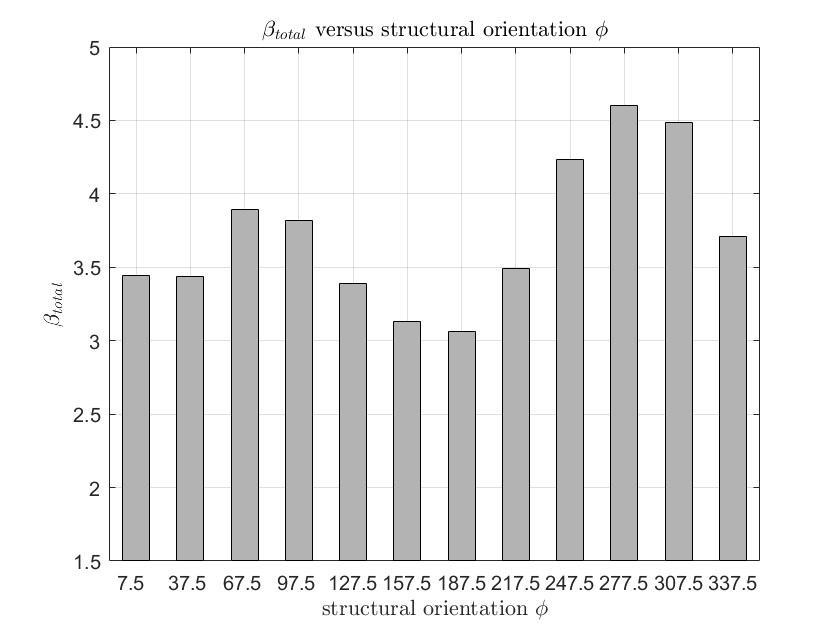
\includegraphics[scale=0.4]{images/beta_total_orientation_G}
		\caption{$\beta_{total}$-values versus building orientation $\phi$ \textcolor{white}{$\beta_{total}$-values versus building orientation $\phi$} \textcolor{white}{$\beta_{total}$-values versus building orientation $\phi$}}
		\label{fig:total_reliability_all_directiosn}
	\end{minipage}
	\hspace{0.4cm}
	\begin{minipage}[]{0.5\textwidth}
		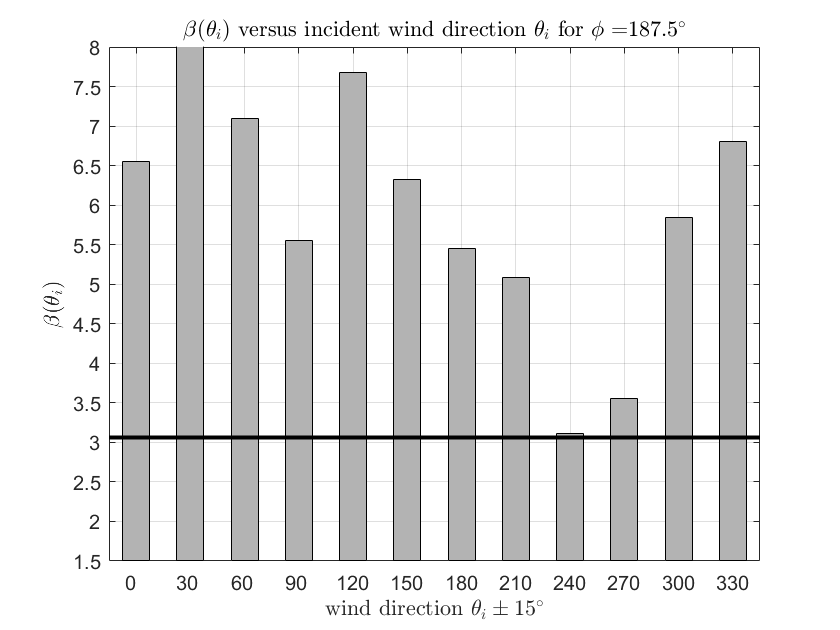
\includegraphics[scale=0.4]{images/unconditional_beta_values_G}
		\caption{Direction-dependent unconditional $\beta$-values versus incident wind-direction $\theta_i$, for building oriention $\phi=187.5^{\circ}$} \label{fig:direction_dependent_beta_values}
	\end{minipage}
\end{figure}

\begin{table}[htb!]
	\centering
	\caption{Averaged $\alpha$-values for all incident wind directions and all orientations of the building}
	\label{alpha-values}
	\begin{tabular}{|l|l|l|}
		\hline
		parameter              & $\mu$ & $\sigma$ \\ \hline
		$\alpha_R$    & 0.22 & 0.01  \\ \hline
		$\alpha_{v_{hr,N}}$             & -0.83 & 0.02  \\ \hline
		$\alpha_{\hat{c}_{pe,hr}}$      & -0.32 & 0.05  \\ \hline
		$\alpha_{c_r^2}$                & -0.33 & 0.01  \\ \hline
		$\alpha_{\chi_{model}}$         & -0.20 & 0.01  \\ \hline
	\end{tabular}
\end{table}

\section{Discussion}\label{discussion}
\textit{Discussion of case-study results}\\
The results show that, due to the wind-directionality effects, the  structural reliability of wind-loaded fa\c{c}ade elements is strongly dependent on the building-orientation, resulting in $\beta_{total}$ values between $3.1\leq\beta_{total}\leq4.6$. In case the wind-directionality effects would not have been taken into account, the outcome of the reliability analysis would be independent of the building orientation and furthermore lower. Especially for the non-governing building orientations this would result in too conservative estimations of the structural reliability. Accounting for wind-directionality effects in the assessment of fa\c{c}ade elements may therefore be extremely advantageous for the design. Similar conclusions have been drawn by Davenport (1983) and Simiu and Filliben (1981).  \\
\\
Furthermore it was found that the total failure probability was almost fully determined by the governing incident wind-directions only; the failure probabilities due to all other incident wind-directions were found to be negligibly small. These results provide arguments for the development of a more practical assessment procedure in the future, where the structural reliability of the fa\c{c}ade element is assessed on the basis of the governing incident wind-directions only. \\
\\
\textit{Discussion of assessment procedure}\\
Even though the results of the case study give good insight in the wind-directionality effects, there are still some remarks to be made concerning the assessment procedure as such. \\
\\
Due to the limited duration of both the wind speed and the wind-tunnel measurements,  the number of sample data available for distribution fitting is relatively small. This introduces large statistical uncertainties in the estimation of the model parameters, which has been shown by Simiu et al. (1978) and Rojiani and Wen (1980). For a better estimation of the structural reliability these statistical uncertainties need to be incorporated in the assessment procedure. \\
\\
Furthermore, for both the extreme wind speeds and the extreme pressure coefficients, the Gumbel fit showed discrepancies with the sample data in the higher probability fractiles. Especially in the case of the extreme pressure coefficients the Gumbel distribution results in a too conservative tail-behaviour. This was also remarked by Kasperski (2003).
In order to assess this discrepancy the distribution skewness is compared with the sample skewness. The sample skewness provides information on the tail behaviour of the random variable, as it is very sensitive for extreme deviations from the mean. In case of the extreme pressure coefficients the sample skewness was found to vary between $-1.65 \leq \hat{\alpha}_c \leq 0.16$. In case of the extreme wind speeds the sample skewness was found to vary between $0.44 \leq \hat{\alpha}_v \leq 1.56$. The  distribution skewness of the Gumbel distribution, however, is fixed to 1.14 for maxima and -1.14 for minima. In many cases this fixed distribution skewness lies far away from the observed sample skewness, explaining the poor fit in the tail.
A better agreement between the sample skewness and the distribution skewness could be obtained the application of a distribution function with a non-fixed distribution skewness, for example the three parameter lognormal distribution or the Weibull distribution. A second option could be the application of a distinct statistical method for the modeling of the extremes, for example the peak-over-threshold method.\\
\\
The structural resistance $R$ was modeled as a lognormally distributed stochastic random variable with a coefficient of variation of $\text{V}_R=0.1$. The design-resistance $R_d$ was assumed to correspond to the EN1990 Level I probability of non-exceedance, with associated sensitivity factor $\alpha_R=0.8$. This chosen sensitivity factor lies far away from the observed sensitivity factor  $\alpha_R=0.22$, which is to be explained by the large uncertainties in the wind-loading part.
For the further development of the assessment procedure it is  recommended to use realistic resistance models for different failure mechanisms and different material types. In this way less assumptions need to be made concerning the design-values of the resistance parameters, as these are fixed according to their characteristic values and partial factors. \\
\\
Finally it is recommended to do further research in the probabilistic modeling of the roughness factor $c_r$ and the model uncertainty factor $\chi_{model}$, which are currently modeled on the basis of approximate literature only. 

\section{Conclusion}\label{conclusions}
In this research an assessment procedure is developed which is able to determine the structural reliability of wind-loaded fa\c{c}ade elements in terms of the failure probability. The assessment procedure accounts for the uncertainties in the extreme wind speeds, the extreme pressure coefficients, the factor correcting for terrain roughness, the structural resistance and the uncertainties in the wind-load model as such. For the modeling of the extreme wind speeds and the extreme pressure coefficients location-specific wind speed and pressure coefficient measurements are being used. The assessment procedure accounts explicitly for the effects of wind-directionality. \\
\\
In order to show its potential, the assessment procedure is applied on a case-study. It is found that the structural reliability of wind-loaded fa\c{c}ade elements is strongly dependent on the building orientation, differing in failure probabilities of several orders of magnitude. Additionally it is found that the failure probability is almost fully determined by the governing incident wind-directions only; the contribution of all other incident wind-directions were found to be negligibly small. \\
\\
For the future developments of the assessment procedure it is recommended to further investigate appropriate statistical methods for the modeling of the extreme wind speeds and the extreme pressure coefficients, to additionally account for the sampling uncertainties in the modeling of the extreme wind speeds and the extreme pressure coefficients, to use realistic resistance models for different failure mechanisms and different material types and, finally, to further investigate the probabilistic description of the roughness factor and the model uncertainty factor.


\nocite{*}
\bibliographystyle{plain}
\bibliography{References}




%
%
%\end{document}

